\documentclass{bmvc2k}

% Any macro definitions you would like to include
% These are not defined in the style file, because they don't begin
% with \bmva, so they might conflict with the user's own macros.
% The \bmvaOneDot macro adds a full stop unless there is one in the
% text already.
\def\eg{\emph{e.g}\bmvaOneDot}
\def\Eg{\emph{E.g}\bmvaOneDot}
\def\etal{\emph{et al}\bmvaOneDot}

\usepackage[]{graphicx}
\usepackage{times}
\usepackage{epsfig}
\usepackage{amsmath}
\usepackage{amssymb}
\usepackage{tabularx}
\usepackage{array}
\usepackage{rotating}
\usepackage{color}
\usepackage{enumerate}
\usepackage{booktabs}
\captionsetup[subfigure]{labelformat=empty}  % remove (a),(b) etc subfloat labels

\newcommand\todo[1]{\textcolor{red}{todo: #1}}
\newcommand\aaron[1]{\textcolor{red}{\bf[Aa: #1]}}
\newcommand\aseem[1]{\textcolor{BrickRed}{aseem: #1}}
\newcommand\holger[1]{\textcolor{Cerulean}{holger: #1}}
\newcommand{\fakebox}[2]{% #1 = width, #2 = height
  {\fboxsep=-\fboxrule\fbox{\rule{0pt}{#2}\rule{#1}{0pt}}}}
\def\httilde{\mbox{\tt\raisebox{-.5ex}{\symbol{126}}}}

\begin{document}

%%%
% BMVC submission: Title, Abstract, Main
% BMVC supplementary materials: Title_Supp, TOC, Supp
% arXiv submission: Title, Abstract, Main, Supp
\newif\ifsupp
\suppfalse  % CHANGE ME

% Title
\ifsupp
    \title{Recognizing Image Style: Supplementary Materials}
    \runninghead{Karayev et al.}{Recognizing Image Style: Supplementary}
\else
    \title{Recognizing Image Style}
    \runninghead{Karayev et al.}{Recognizing Image Style}
\fi
\def\httilde{\mbox{\tt\raisebox{-.5ex}{\symbol{126}}}}
\addauthor{Sergey Karayev}{}{1}
\addauthor{Matthew Trentacoste}{}{2}
\addauthor{Helen Han}{}{1}
\addauthor{Aseem Agarwala}{}{2}
\addauthor{Trevor Darrell}{}{1}
\addauthor{Aaron Hertzmann}{}{2}
\addauthor{Holger Winnemoeller}{}{2}
\addinstitution{University of California, Berkeley}
\addinstitution{Adobe}

\maketitle

\ifsupp
    \listoffigures
    \listoftables
\else
    \begin{abstract}
    The style of an image plays a significant role in how it is viewed, but style has received little attention in computer vision research.
We describe an approach to predicting style of images, and perform a thorough evaluation of different image features for these tasks.
We find that features learned in a multi-layer network generally perform best -- even when trained with object class (not style) labels.
Our large-scale learning methods results in the best published performance on an existing dataset of aesthetic ratings and photographic style annotations.
We present two novel datasets: 80K Flickr photographs annotated with 20 curated style labels, and 85K paintings annotated with 25 style/genre labels.
Our approach shows excellent classification performance on both datasets.
We use the learned classifiers to extend traditional tag-based image search to consider stylistic constraints, and demonstrate cross-dataset understanding of style.

    \end{abstract}

    

\begin{figure}[ht!]
\centering
\subfloat[][HDR]{\includegraphics[width=\samplewidth]{../arxiv/figures/flickrDatasetExamples/9566063566_a26f090068.jpg}}~
\subfloat[][Long Exposure]{\includegraphics[width=\samplewidth]{../arxiv/figures/flickrDatasetExamples/9558960217_7056981249.jpg}}~
\subfloat[][Macro]{\includegraphics[width=\samplewidth]{../arxiv/figures/flickrDatasetExamples/9550304852_99568eec75.jpg}}
\vspace{-2ex}

\subfloat[][Vintage]{\includegraphics[width=\samplewidth]{../arxiv/figures/flickrDatasetExamples/5863276871_8bf39b0177_crop.jpg}}~
\subfloat[][Romantic]{\includegraphics[width=\samplewidth]{../arxiv/figures/flickrDatasetExamples/8546146794_a60b92a504.jpg}}~
\subfloat[][Horror]{\includegraphics[width=\samplewidth]{../arxiv/figures/flickrDatasetExamples/3444380200_0941a7ce5b.jpg}}
\vspace{-2ex}

\subfloat[][Minimal]{\includegraphics[width=\samplewidth]{../arxiv/figures/flickrDatasetExamples/9039257065_8a87e1f3f6.jpg}}~
\subfloat[][Hazy]{\includegraphics[width=\samplewidth]{../arxiv/figures/flickrDatasetExamples/6588242067_c0a74e7da0.jpg}}~
\subfloat[][Noir]{\includegraphics[width=\samplewidth]{../arxiv/figures/flickrDatasetExamples/3427272477_444a9a038d.jpg}}
%\vspace{-2ex}

\caption{
    Typical images in different style categories of our Flickr Style dataset.
    The dataset comprises 18 styles in total, each with 3,000 examples.
}
\label{fig:flickr_style_examples}
\end{figure}
\section{Introduction}

Images convey meaning in multiple ways; \textit{visual style} is often a significant component of image meaning for creative images.
For example, the same scene portrayed in
the lush, springtime colors of a Renoir painting would tell a different story than shown in the harsh, dark tones of a typical horror movie.
Visual style is crucial to how a viewer interprets an image in many contexts, including art, design, entertainment, advertising, and social media.
%It plays a major role in creative tasks such as illustrating articles, presentations, creating and editing photographs, and other design work.
Moreover, an increasing amount of visual media consumption though online social media feeds, photo sharing sites, and news sites,
is now curated by machines and not people.
%Indeed, automatic approaches (such as Google+ Photos) now edit and even create visual content from source materials.
Yet, virtually no research in computer vision has explored visual style.

This paper introduces new approaches and datasets for the automatic analysis of image style.
Visual style is very recognizable to human viewers, yet difficult to define precisely. Style may combine aspects of color, lighting, composition, scene objects, and other facets. Hence, we prefer to define style empirically through labelled data, and then analyze the divisions between these classes.
Finding existing datasets insufficient, %\holger{I assume we expand this in the related work section. I.e. which datasets we are referring to and why they are insufficient},
we gather a new large-scale dataset of photographs annotated with diverse visual style labels.
This dataset embodies several different aspects of visual style, including photographic techniques (``Macro," ``HDR"), composition styles (``Minimal," ``Geometric"),
moods (``Serene," ``Melancholy"), genres (``Vintage," ``Romantic," ``Horror"),
and types of scenes (``Hazy,'' ``Sunny''). %\holger{I do remember an early discussion on style classification versus scene classification. Is it really different? I imagine the machinery to distinguish a beach image from a cityscape, from a forest picture, from a portrait is quite similar to our style detection machinery. If so, what is different? Are we discussing this in the related work section?}
We  also gather a large dataset of visual art (mostly paintings) annotated with art historical style labels, ranging from Renaissance to modern art.
We perform a thorough evaluation of different visual features for the task of predicting these style annotations.
We find that ``deep'' features trained on a large amount of data labeled with object class categories (ImageNet) perform significantly better than traditionally used hand-designed features.

The style predictors that our datasets and learning enable are useful as mid-level features in their own right.
When making presentations, a searchable source of stylistically coherent images would be useful.
A story may be illustrated with images that match not only its objective content, but also its sentiment.
In addition to evaluating classification performance of our approach, we demonstrate an application of style classifiers to visual search, making a large image collection searchable by both content tags and visual style (``bird, bright/energetic," ``train, film noir").
Additionally, we demonstrate that styles learned from paintings can be used to search collections of photographs, and vice versa.

%Additionally, we enable visual similarity search results to be filtered by visual style, making possible queries such as ``similar to this image, but scarier''.

All data, trained predictors, code, and a web-based user interface for searching image collections ``with style'' will be released upon publication.

\begin{figure} %[ht]
\centering

\subfloat[][Baroque]{\includegraphics[width=\samplewidth]{../arxiv/figures/wikipaintingsDatasetExamples/adriaen-van-de-velde-battle.jpg}}~
\subfloat[][Rococo]{\includegraphics[width=\samplewidth]{../arxiv/figures/wikipaintingsDatasetExamples/william-hogarth-after-outdoor-scene-crop.jpg}}~
\subfloat[][Northern Renaissance]{\includegraphics[width=\samplewidth]{../arxiv/figures/wikipaintingsDatasetExamples/jan-van-hemessan-a-merry-company.jpg}}
\vspace{-2ex}

\subfloat[][Impressionism]{\includegraphics[width=\samplewidth]{../arxiv/figures/wikipaintingsDatasetExamples/a-bar-at-the-folies-bergere-1882-1.jpg}}~
\subfloat[][Post-Impressionism]{\includegraphics[width=\samplewidth]{../arxiv/figures/wikipaintingsDatasetExamples/a-breton-landscape-david-s-mill-1894.jpg}}~
%\subfloat[][Surrealism]{\includegraphics[width=\samplewidth]{a-dew-drop-falling-from-a-bird-s-wing-wakes-rosalie-who-has-been-asleep-in-the-shadow-of-a.jpg}
\subfloat[][Ukiyo-e]{\includegraphics[width=\samplewidth]{../arxiv/figures/wikipaintingsDatasetExamples/asakusa-honganji-temple-in-th-eastern-capital.jpg}}
%\subfloat[][Cubism]{\includegraphics[width=\samplewidth]{picasso-algerian-women-delacroix-1955.jpg}
\vspace{-2ex}

\subfloat[][Abs.~Expressionism]{\includegraphics[width=\samplewidth]{../arxiv/figures/wikipaintingsDatasetExamples/elaine-de-kooning-abstract-1970.jpg}}~
\subfloat[][Minimalism]{\includegraphics[width=\samplewidth]{../arxiv/figures/wikipaintingsDatasetExamples/4-rythmes-interf-rents-en-formant-un-carr-1972.jpg}}~
\subfloat[][Color Field Painting]{\includegraphics[width=\samplewidth]{../arxiv/figures/wikipaintingsDatasetExamples/leon-berkowitz-after-the-cloud.jpg}}
\vspace{-2ex}

\caption{
    Typical images in different style categories from our Wikipaintings dataset.
    The dataset comprises 85,000 images labeled with 22 art historical styles.
}
\label{fig:wikipaintings_examples}
\end{figure}

    %!TEX root = paper/paper.tex
\section{Related Work}

Most research in computer vision addresses recognition and reconstruction, independent of image style.
A few previous works have focused directly on image composition, particularly on the high-level attributes of beauty, interestingness, and memorability.

Most commonly, several previous authors have described methods to predict aesthetic quality of photographs.
Datta et al.~\cite{Datta-ECCV-2006}, designed visual features to represent concepts such as colorfulness, saturation, rule-of-thirds, and depth-of-field, and evaluated aesthetic rating predictions on photographs; The same approach was further applied to a small set of Impressionist paintings~\cite{Li-SP-2009}.
The feature space was expanded with more high-level descriptive features such as ``presence of animals'' and ``opposing colors'' by Dhar et al., who also attempted to predict Flickr's proprietary ``interestingness'' measure, which is determined by social activity on the website~\cite{Dhar-CVPR-2011}.
Gygli et al.~\cite{Gygli-ICCV-2013} gathered and predicted human evaluation of image interestingness, building on work by Isola et al.~\cite{Isola-CVPR-2011}, who used various high-level features to predict human judgements of image memorability.
In a similar task, Borth et al.~\cite{Borth-MM-2013} performed sentiment analysis on images using object classifiers trained on adjective-noun pairs.
% Gemert \cite{gemert2011} compares the similarity between two image compositions based on spatial pyramid similarity.

Murray et al.~\cite{Murray-CVPR-2012} introduced the Aesthetic Visual Analysis (AVA) dataset, annotated with ratings by users of DPChallenge, a photographic skill competition website.
The AVA dataset contains some photographic style labels (e.g., ``Duotones,'' ``HDR''), derived from the titles and descriptions of the photographic challenges to which photos were submitted.
Using images from this dataset, Marchesotti and Peronnin~\cite{Marchesotti-BMVC-2013} gathered bi-grams from user comments on the website, and used a simple sparse feature selection method to find ones predictive of aesthetic rating.
The attributes they found to be informative (e.g., ``lovely photo,'' ``nice detail'') are not specific to image style.

Several previous authors have developed systems to classify classic painting styles, including \cite{keren2002,shamir2010}.
These works consider only a handful of styles (less than ten apiece), with styles that are visually very distinct, e.g., Pollock vs.~Dal\'{\i}.
These datasets comprise less than 60 images per style, for both testing and training.
Mensink \cite{Mensink2014} provides a larger dataset of artworks, but does not consider style classification.

    
\section{Data Sources}

%The computer vision community has made impressive progress in scene and object recognition due in  part to the increasing quality of training data, and it has been shown numerous times that performance increases with the amount of labeled data.
Performance of scene and object recognition depends directly on the quality of the training data set.
To our knowledge, there is only one existing dataset annotated with visual style, and only a narrow range of styles are represented~\cite{Murray-CVPR-2012}. % \holger{I assume we are referring to AVA, so should we use \cite{Murray-CVPR-2012} here?}.
%However, there are practically no datasets with annotated visual style, and the existing ones are very small.
We review the best current dataset for aesthetic prediction, which has a subset of style annotations.
We then present two new datasets, covering a range of visual styles.
% one of photographs, the other of paintings. %\holger{Why? Maybe
% say that photographs are so abundant and therefore (a) easy
% to come by and (b) relevant for applications; and for paintings:
% That they generally tend to have much stronger stylistic
% attributes than the general photograph. At this point, we
% should think about whether we want to discuss the aspect of
% quality... i.e. a professional photographer may use style in
% a very similar way that a painter does, but John Doe on the
% street would not. This affects the quality of the datasets we
% use. My suggestion: We shouldn’t go into too much detail
% here, but we should at least give a brief explanation of why
% we choose the datasets we did and why we consider this a
% good choice.}

\subsection{Aesthetic Visual Analysis (AVA)}

AVA \cite{Murray-CVPR-2012}  is a dataset of 250K images from \url{dpchallenge.net}, where users submit and judge photos organized into thematic challenges such as ``Cats'', ``Textures and Materials'', or ``Depth of Field''.
On average, an image receives around 200 ratings on a 1-10 scale.
These ratings reflect both absolute image quality and how well the image meets the goals of the specific challenge.
The dataset also includes 14,000 images annotated with 14 labels of photographic style, manually created by the authors by combining photos from 72 different challenges.
The task in this dataset is to predict rating mean and standard deviations, and to predict style labels. The authors did not report prediction scores on style prediction.

The styles in AVA are primarily photographic techniques, such as ``HDR'' and ``Long Exposure," and simple compositional techniques such as ``Silhouettes," and ``Vanishing Point."
Out of the 14 photographic style labels, less than half have over a thousand positive examples, and ``higher-level" styles such as mood and genre styles are not represented.

%We evaluate on the published tasks of classifying whether the mean of the ratings distribution (beauty) of an image is above the global mean, and classifying the presence of any of the photographic style labels.
%Additionally, we classify whether the standard deviation of the ratings distribution (opinion polarization) of an image is above the global mean.
% , and evaluate regression as well as classification performance on the mean and standard deviation prediction tasks.
%Following the observation that some challenges have lower average ratings than others, we also predict challenge-normalized ratings mean and standard deviation.}

\subsection{Flickr and Pinterest Style}

Our goal is to describe a broader range of image style beyond photographic style, which also includes a range of genres, compositional styles, and moods.
We would like to gather data from a rich source, so that the size of our dataset can be increased with minimal effort.
We consider two sources: Flickr and Pinterest.

\paragraph{Flickr}
Although Flickr users often provide free-form tags for their uploaded images, the tags tend to be quite unreliable.
Instead, we turn to Flickr groups, which are community-curated collections of visual concepts.
There are active, well-populated Flickr Groups for most visual style concepts that we considered.

We selected 20 groups with large image collections and clearly defined membership rules to produce our Flickr Style dataset.
We collected 4,000 positive examples for each label, for a total of 80,000 images.
Example images are shown in \autoref{fig:flickr_style_examples}, and examples of the group rules and image counts are given in \autoref{tab:flickr_style}.
The names of the 20 styles can be seen in the confusion matrix (\autoref{fig:flickr_confusion}) and in \autoref{tab:flickr_aps}.



\begin{table}
\caption {Sample of our Flickr Style groups, showing the size of available data and the membership rules.}
\label{tab:flickr_style}
{\small
    \begin{tabularx}{\linewidth}{m{2.3cm}rX}
    \textbf{Group (Style)}       & \textbf{Images} & \textbf{Description (excerpt)}                                                                                                                                                                             \\ \hline
    Geometric Beauty (Geometric) & 153909           & Circles, triangles, rectangles, symmetric objects, repeated patterns ...                                                                                            \\
    Pastel, Soft (Pastel)    & 100116           & Pastels and whites, blossom and sunglares. Anything that is soft, pretty and just dreamy.                                             \\
    Film Noir Mood  (Noir) & 7775             & Not just black and white photography, but a dark, gritty, moody feel. ... \\
    Horror (Horror)          & 16501            & The scariest pics you can find. ... your bloodiest, ghastliest, freakiest snaps. ...                       \\
    Melancholy (Melancholy)      & 90748            & Only melancholic shots.                                                                                                                                                                           \\
    \end{tabularx}
}
\end{table}


\paragraph{Pinterest}
On Pinterest, users create their own private boards, which are often dedicated to a single stylistic concept, such as ``Macro Photography'' or ``Ethereal''.
The breadth of such concepts is quite astounding --- there are hundreds of boards for individual designers, schools of design, abstract concepts, etc.

We search Pinterest boards for each one of our 20 styles, and fetch at most 500 boards for each style.
Each board has on average 60 pins, for a total of 600,000 pins.
This dataset is downsampled to 80,000 to exactly match the size of the Flickr dataset.

\paragraph{Negative labels}
On both these datasets, the labels are considered clean in the positive examples, but noisy in the negative examples, in the same way as the ImageNet dataset \cite{Deng-CVPR-2009}.
That is, a picture labeled as \emph{Sunny} is indeed \emph{Sunny}, but it may also be \emph{Romantic}, for which it is not labeled.
Following ImageNet, we still treat the absence of a label as indication that the image is a negative example for that label.
We consider this an unfortunate but acceptable reality of working with a large-scale dataset.

\todo{Discussion of human performance verification using MechTurk should go here.}

\subsection{Wikipaintings}
The above datasets deal exclusively with modern, photographic images.
To our knowledge, no existing vision algorithm can categorize non-photorealistic media, such as paintings and drawings.
In a major step to this goal, we collect a dataset of 100,000 high-art images -- mostly paintings -- labeled with artist, style, genre, date, and free-form tag information by a community of experts on the Wikipaintings website.

% \holger{Additional points we could make: Paintings are older
% than photographs and much of what we know about
% styles was developed in painting (or other visual media) before
% it was applied in photography. We can say that the
% style in paintings is often very refined, and we can say that
% the painting datasets have a lot of useful and complete metadata
% attached.}
%
%In order to analyze the style of non-photorealistic media,
%We would also like to model the style of non-photorealistic media from historical sources.
%What about the large corpus of visual media produced over the centuries: drawings, paintings, engravings, etc.?
%We would like to be able to discuss their visual style as well.

Analyzing style of non-photorealistic media is an interesting problem, as much of our present understanding of visual style arises out of thousands of years of developments in fine art, marked by distinct historical styles.
As shown in~\autoref{fig:wikipaintings_data}, the dataset presents significant stylistic diversity, primarily spanning Renaissance styles to modern art movements.
We select 22 styles with more than 1,000 examples, for a total of 85,000 images.
Example images are shown in~\autoref{fig:wikipaintings_examples}.

\begin{figure}[th]
\centering
\includegraphics[width=.9\linewidth]{../arxiv/figures/wikipaintings_style.pdf}\\
\includegraphics[width=.9\linewidth]{../arxiv/figures/wikipaintings_genre.pdf}\\
\includegraphics[width=.9\linewidth]{../arxiv/figures/wikipaintings_date.pdf}
\caption{Distribution of image style, genre, and date in the Wikipaintings dataset.}
\label{fig:wikipaintings_data}
\end{figure}

    %!TEX root = paper/paper.tex
\section{Learning algorithm}

We learn to classify novel images according to their style, using the labels assembled in the previous section.
Because the datasets we deal with are quite large and some of the features are high-dimensional, we consider only linear classifiers, relying on sophisticated features to provide robustiness.

We use an open-source implementation of Stochastic Gradient Descent with adaptive subgradient \cite{Agarwal-JMLR-2012}.
The learning process optimizes the function \[
\underset{w}{\text{min }} \lambda_1 \|w\|_1 + \frac{\lambda_2}{2} \Vert w \Vert_2^2 + \sum_i \ell(x_i, y_i, w)
\]
We set the $L_1$ and $L_2$ regularization parameters and the form of the loss function by validation on a held-out set.
For the loss $\ell(x, y, w)$, we consider the hinge ($\max(0, 1 - y \cdot w^T x)$) and logistic ($\log(1 + \exp(-y \cdot w^T x))$) functions.
We set the initial learning rate to $0.5$, and use adaptive subgradient optimization~\cite{duchi2011adaptive}.
Our setup is of multi-class classification; we use the One vs. All reduction to binary classifiers.

    %!TEX root = paper/paper.tex
\section{Image Features}

In order to classify styles, we must choose appropriate image features.  We hypothesize that image style may be related to many different features, including low-level statistics \cite{Lyu-PNAS-2004}, color choices, composition, and content.  Hence, we test features that embody these different elements, including features from the object recognition literature.
We evaluate single-feature performance, as well as second-stage fusion of multiple features.

\vspace{-1em}
\paragraph{L*a*b color histogram.}
Many of the Flickr styles exhibit strong dependence on color. For example, \emph{Noir} images are nearly all black-and-white, while most \emph{Horror} images are very dark, and \emph{Vintage} images use old photographic colors. We use a standard color histogram feature, computed on the whole image.
The 784-dimensional joint histogram in CIELAB color space has 4, 14, and 14 bins in the L*, a*, and b* channels, following Palermo et al.~\cite{Palermo-ECCV-2012}, who showed this to be the best performing single feature for determining the date of historical color images.

\vspace{-1em}
\paragraph{GIST.}
The classic gist descriptor \cite{Oliva-IJCV-2001} is known to perform well for scene classification and retrieval of images visually similar at a low-resolution scale, and thus can represent image composition to some extent.
We use the INRIA LEAR implementation, resizing images to 256 by 256 pixels and extracting a 960-dimensional color GIST feature.

\vspace{-1em}
\paragraph{Graph-based visual saliency.}
We also model composition with a visual attention feature \cite{Harel-NIPS-2006}.
The feature is fast to compute and has been shown to predict human fixations in natural images basically as well as an individual human (humans are far better in aggregate, however).
The 1024-dimensional feature is computed from images resized to 256 by 256 pixels.

\vspace{-1em}
\paragraph{Meta-class binary features.}
Image content can be predictive of individual styles, e.g., \emph{Macro} images include many images of insects and flowers. The \texttt{mc-bit} feature~\cite{Bergamo-CVPR-2012} is a 15,000-dimensional bit vector feature learned as a non-linear combination of classifiers trained using existing features (e.g., SIFT, GIST, Self-Similarity) on thousands of random ImageNet synsets, including internal ILSVRC2010 nodes.
In essence, MC-bit is a hand-crafted ``deep'' architecture, stacking classifiers and pooling operations on top of lower-level features.

\vspace{-1em}
\paragraph{Deep convolutional net.}
Current state-of-the-art results on ImageNet, the largest image classification challenge, have come from a deep convolutional network trained in a fully-supervised manner \cite{krizhevsky2012imagenet}.
We use the Caffe \cite{Jia13caffe} open-source implementation of the ImageNet-winning eght-layer convolutional network, trained on over a million images annotated with 1,000 ImageNet classes.
We investigate using features from two different levels of the network, referred to as DeCAF$_5$ and DeCAF$_6$ (following \cite{Donahue2013}).
The features are 8,000- and 4,000-dimensional and are computed from images center-cropped and resized to 256 by 256 pixels.
% Since DeCAF is trained on object recognition, not style recognition, we also test whether tuning the network for our style datasets improve performance.

\vspace{-1em}
\paragraph{Content classifiers.}
Following Dhar et al.~\cite{Dhar-CVPR-2011}, who use high-level classifiers as features for their aesthetic rating prediction task, we evaluate using object classifier confidences as features.
Specifically, we train classifiers for all 20 classes of the PASCAL VOC \cite{pascal-voc-2010} using the DeCAF$_6$ feature.
The resulting classifiers are quite reliable, obtaining $0.7$ mean AP on the VOC 2012.

We aggregate the data to train four classifiers for ``animals'', ``vehicles'', ``indoor objects'' and ``people''.
These aggregate classes are presumed to discriminate between vastly different types of images -- types for which different style signals may apply.
For example, a \emph{Romantic} scene with people may be largely about the composition of the scene, whereas, \emph{Romantic} scenes with vehicles may be largely described by color.
%An example about predicting Romantic style: for a picture with people, scene composition may be key, but for a picture with vehicles, color scheme may be most important.

To enable our classifiers to learn content-dependent style, we can take the outer product of a feature channel with the four aggregate content classifiers.

    %!TEX root = paper/paper.tex
\section{Experiments}

% Details of our experiments follow, with a concluding discussion section.
% Due to space constraints, we are not able to provide as many figures as we would like here; however, the Supplementary Materials provides a full accounting.

\begin{table}
\caption{
    Mean APs on three datasets for the considered single-channel features and their second-stage combination.
    As some features were clearly worse than others on the AVA Style dataset, only the better features were evaluated on larger datasets.
}
\label{tab:mean_aps}
\centering
\vspace{1em}
\footnotesize{
\begin{tabular}{lrrrrrrrrr}
\toprule
{}                & Fusion x Content & DeCAF$_6$ & MC-bit & L*a*b* Hist & GIST  & Saliency & random \\
\midrule
AVA Style         & \textbf{0.581}   & 0.579     & 0.539  & 0.288       & 0.220 & 0.152    & 0.132 \\
Flickr            & \textbf{0.368}   & 0.336     & 0.328  & -           & -     & -        & 0.052 \\
Wikipaintings     & \textbf{0.473}   & 0.356     & 0.441  & -           & -     & -        & 0.043 \\
\bottomrule
\end{tabular}
}
\end{table}


\subsection{Flickr Style}
We learn and predict style labels on the 80,000 images labeled with 20 different visual styles of our new Flickr Style dataset, using 20\% of the data for testing, and another 20\% for parameter-tuning validation.

There are several performance metrics we consider.
Average Precision evaluation (as reported in \autoref{tab:mean_aps} and in detailed tables in the Supplementary Materials) is computed on a random class-balanced subset of the test data (each class has equal prevalence).
We compute confusion matrices on the same data.
Per-class accuracies are computed on subsets of the data balanced by the binary label, such that chance performance is 50\%.
We follow these decisions in all following experiments.

The best single-channel feature is DeCAF$_6$ with 0.336 mean AP; feature fusion obtains 0.368 mean AP.
Per-class APs range from 0.17 [Depth of Field] to  0.62 [Macro].
Per-class accuracies range from 68\% [Romantic, Depth of Field] to 85\% [Sunny, Noir, Macro].
The average per-class accuracy is 78\%.
We show the most confident style classifications on the test set of Flickr Style in \autoref{fig:flickr_on_flickr}.

Upon inspection of the confusion matrices, we saw points of understandable confusion: Depth of Field vs.~Macro, Romantic vs.~Pastel, Vintage vs.~Melancholy.
There are also surprising sources of mistakes: Macro vs.~Bright/Energetic, for example.
To explain this particular confusion, we observed that lots of Macro photos contain bright flowers, insects, or birds, often against vibrant greenery.
Here, at least, the content of the image dominates its style label.

To explore further content-style correlations, we plot the outputs of PASCAL object class classifiers (one of our features) on the Flickr dataset in~\autoref{fig:content_correlation}.
We can observe that some styles have strong correlations to content (e.g., ``Hazy'' occurs with ``vehicle'', ``HDR'' doesn't occur with ``cat'').

We hypothesize that style is content-dependent: a Romantic portrait may have different low-level properties than a Romantic sunset. We form a new feature as an outer product of our content classifier features with the second-stage late fusion features (``Fusion $\times$ Content'' in all results figures).  These features gave the best results, thus supporting the hypothesis.

\begin{figure}[h]
\centering
    \includegraphics[width=\linewidth]{../../figures/content_correlation2/pascal_on_flickr.pdf}
    \caption{
        Correlation of PASCAL content classifier predictions (rows) against ground truth Flickr Style labels (columns).
        We see, for instance, that the Macro style is highly correlated with presence of animals, and that Long Exposure and Sunny style photographs often feature vehicles.
    }\label{fig:content_correlation}
\end{figure}

\vspace{-.5em}
\paragraph{Mechanical Turk Evaluation.}\label{sec:mech_turk_evaluation}
In order to provide a human baseline for evaluation, we performed a Mechanical Turk study.
For each style, Turkers were shown positive and negative examples for each Flickr Group, and then they evaluated whether each image in the test set was part of the given style.
We treat the Flickr group memberships as ground truth as before, and then evaluate Turkers' ability to accurately determine group membership.
Measures were taken to remove spam workers; see the Supplemental Material details on the experimental setup.
For efficiency, one quarter of the test set was used, and two redundant styles (Bokeh and Detailed) were removed.
Each test image was evaluated by 3 Turkers, and the majority vote taken as the human result for this image.

In total, Turkers achieved 75\% mean accuracy (ranging from 61\% [Romantic] to 92\% [Macro]) across styles, in comparison to 78\% mean accuracy (ranging from 68\% [Depth of Field] to 87\% [Macro]) of our best method.
Our algorithm did significantly worse than Turkers on Macro and Horror, and significantly better on Vintage, Romantic, Pastel, Detailed, HDR, and Long Exposure styles.

Some of this variance may be due to subtle difference from the Turk tasks that we provided, as compared to the definitions of the Flickr groups, but may also due to the Flickr groups' incorporating images that do not quite fit the common definition of the given style.
For example, there may be a mismatch between different notions of ``romantic'' and ``vintage,'' and how inclusively these terms are defined.

We additionally used the Turker opinion as ground truth for our method's predictions.
In switching from the default Flickr to the MTurk ground truth, our method's accuracy hardly changed from 78\% to 77\%.
However, we saw that the accuracy of our Vintage, Detailed, Long Exposure, Minimal, HDR, and Sunny style classifiers significantly decreased, indicating machine-human disagreement on those styles.
Detailed tables are provided in Supplemental Results.

\subsection{Wikipaintings}
With the same setup and features as in the Flickr experiments, we evaluate 85,000 images labeled with 25 different art styles.
The results are given in \autoref{tab:mean_aps} and in Supplementary Materials.
The best single-channel feature is MC-bit with 0.441 mean AP; feature fusion obtains 0.473 mean AP.
Per-class accuracies range from 72\% [Symbolism, Expressionism, Art Nouveau] to 94\% [Ukiyo-e, Minimalism, Color Field Painting].

\subsection{AVA Style}
AVA \cite{Murray-CVPR-2012} is a dataset of 250K images from \texttt{dpchallenge.net}.
We evaluate classification of aesthetic rating and of 14 different photographic style labels on the 14,000 images of the AVA dataset that have such labels.
For the style labels, the publishers of the dataset provide a train/test split, where training images have only one label, but test images may have more than one label \cite{Murray-CVPR-2012}.
For style classification, the best single feature is the DeCAF$_6$ convolution network feature, obtaining 0.579 mean AP.
Feature fusion improves the result to 0.581 mean AP; both results beat the previous state-of-the-art of 0.538 mean AP \cite{Murray-CVPR-2012}.
% \footnote{Our results beat 0.54 mAP using both the AVA-provided class-imbalanced test split, and the class-balanced subsample that we consider to be more correct evaluation, and for which we provide numbers.}

In all metrics, the DeCAF and MC-bit features significantly outperformed more low-level features on this dataset.
Accordingly, we do not evaluate the low-level features on the larger Flickr and Wikipaintings datasets.

    Test images were grouped into 10 images per Human Interface Task (HIT). Each task asks the Turker to evaluate the style (e.g., ``Is this image VINTAGE?'') for each image.  For each style, we provided a short blurb describing the style in words, and provided 12-15 hand-chosen positive and negative examples for each Flickr Group.
Each HIT included 2 sentinels: images which were very clearly positives and similar to the examples.  HITs were rejected when Turkers got both sentinels wrong.
Turkers were paid $0.10$ per HIT, and were allowed to perform multiple hits.  Manual inspection of the results indicate that the Turkers understood the task and were performing effectively.  A few Turkers sent unsolicited feedback indicating that they were really enjoying the HITs (``some of the photos are beautiful'') and wanted to perform them as effectively as possible.

    %!TEX root = paper/paper.tex
\subsection{Application: Style-Based Image Search}

\newcommand{\fgap}{.6in}
\begin{figure}[h!]
\centering
\begin{tabular}{m{.02in}|m{\fgap} m{\fgap} m{\fgap} m{\fgap} m{\fgap}}
    \begin{turn}{90}\footnotesize{Minimal}\end{turn} &
    \includegraphics[width=.75in]{../../figures/flickr_on_flickr/pred_style_Minimal/w/0.jpg} &
    \includegraphics[width=.75in]{../../figures/flickr_on_flickr/pred_style_Minimal/w/1.jpg} &
    \includegraphics[width=.75in]{../../figures/flickr_on_flickr/pred_style_Minimal/w/2.jpg} &
    \includegraphics[width=.75in]{../../figures/flickr_on_flickr/pred_style_Minimal/w/3.jpg} &
    \includegraphics[width=.75in]{../../figures/flickr_on_flickr/pred_style_Minimal/w/4.jpg} \\
    \begin{turn}{90}\footnotesize{Melancholy}\end{turn} &
    \includegraphics[width=.75in]{../../figures/flickr_on_flickr/pred_style_Melancholy/w/0.jpg} &
    \includegraphics[width=.75in]{../../figures/flickr_on_flickr/pred_style_Melancholy/w/1.jpg} &
    \includegraphics[width=.75in]{../../figures/flickr_on_flickr/pred_style_Melancholy/w/2.jpg} &
    \includegraphics[width=.75in]{../../figures/flickr_on_flickr/pred_style_Melancholy/w/3.jpg} &
    \includegraphics[width=.75in]{../../figures/flickr_on_flickr/pred_style_Melancholy/w/4.jpg} \\
    \begin{turn}{90}\footnotesize{HDR}\end{turn} &
    \includegraphics[width=.75in]{../../figures/flickr_on_flickr/pred_style_HDR/w/0.jpg} &
    \includegraphics[width=.75in]{../../figures/flickr_on_flickr/pred_style_HDR/w/1.jpg} &
    \includegraphics[width=.75in]{../../figures/flickr_on_flickr/pred_style_HDR/w/2.jpg} &
    \includegraphics[width=.75in]{../../figures/flickr_on_flickr/pred_style_HDR/w/3.jpg} &
    \includegraphics[width=.75in]{../../figures/flickr_on_flickr/pred_style_HDR/w/4.jpg} \\
    \begin{turn}{90}\footnotesize{Vintage}\end{turn} &
    \includegraphics[width=.75in]{../../figures/flickr_on_flickr/pred_style_Vintage/w/0.jpg} &
    \includegraphics[width=.75in]{../../figures/flickr_on_flickr/pred_style_Vintage/w/1.jpg} &
    \includegraphics[width=.75in]{../../figures/flickr_on_flickr/pred_style_Vintage/w/2.jpg} &
    \includegraphics[width=.75in]{../../figures/flickr_on_flickr/pred_style_Vintage/w/3.jpg} &
    \includegraphics[width=.75in]{../../figures/flickr_on_flickr/pred_style_Vintage/w/4.jpg} \\
\end{tabular}
\vspace{1em}
\caption{
    Top five most-confident positive predictions on the Flickr Style test set, for a few different styles.
    See Figures 1-3 of the Supplemental Material for more results.
}\label{fig:flickr_on_flickr}
\end{figure}


Style classifiers learned on our datasets can be used toward novel goals.
For example, sources of stock photography or design inspiration may be better navigated with a vocabulary of style.
Currently, companies expend labor to manually annotate stock photography with such labels.
With our approach, any image collection can be searchable and rankable by style.

To demonstrate, we apply our Flickr-learned style classifiers to a new dataset of 80K images gathered on Pinterest (also available with our code release); some results are shown in \autoref{fig:flickr_on_pinterest}.
Interestingly, styles learned from photographs can be used to order paintings, and styles learned from paintings can be used to order photographs, as illustrated in \autoref{fig:photo_painting}.

\begin{figure*}[ht]
\centering
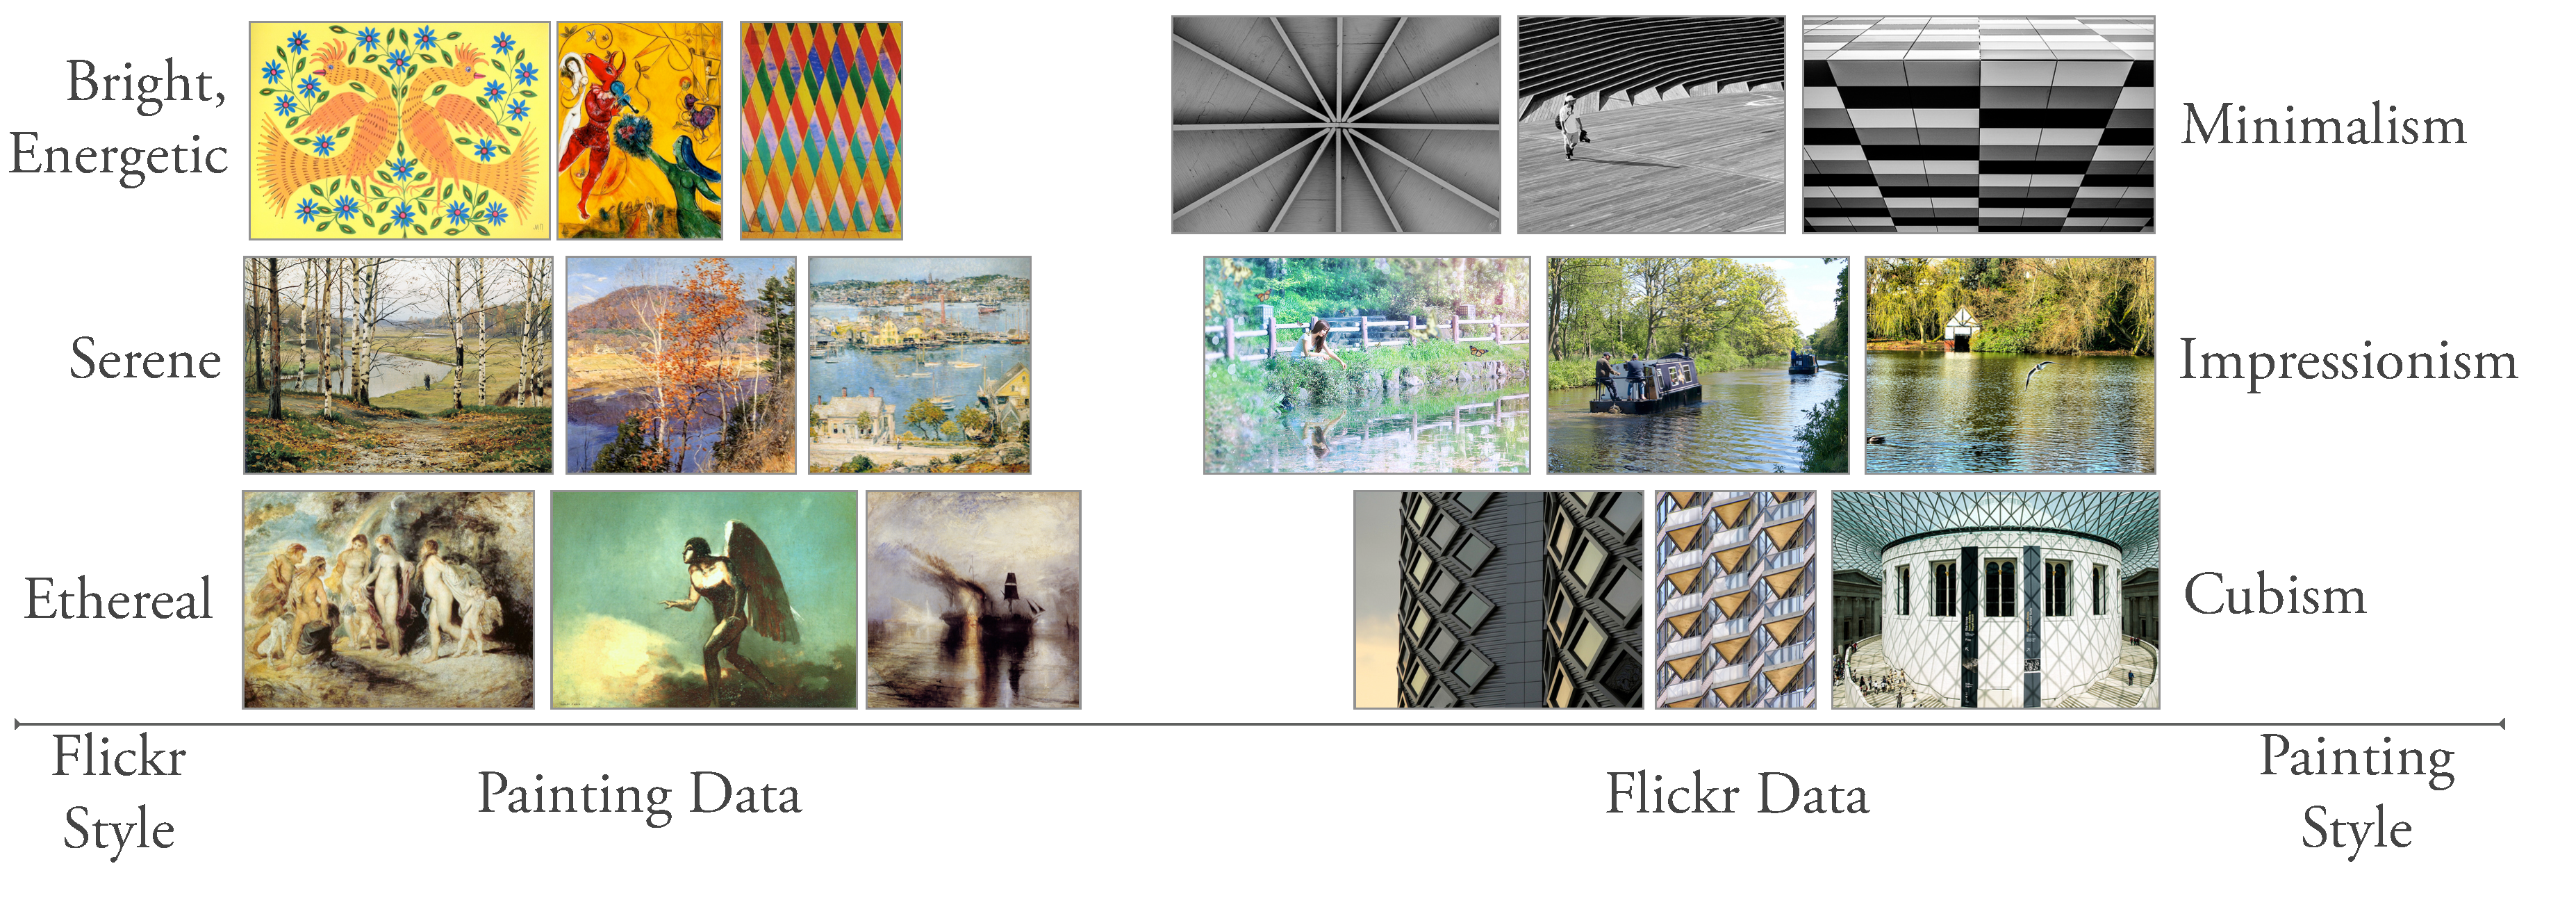
\includegraphics[width=.95\linewidth]{../../figures/style_by_style.pdf}
\vspace{-1ex}
\caption{
    Cross-dataset style.
    On the left are shown top scorers from the Wikipaintings set, for styles learned on the Flickr set.
    On the right, Flickr photographs are accordingly sorted by Painting style.
    (Figure best viewed in color.)
}
\label{fig:photo_painting}
\end{figure*}

\newcommand{\dgap}{.42in}
\begin{figure}
\begin{subfigure}[t]{0.48\linewidth}
    \begin{tabular}{m{.02in}|m{\dgap} m{\dgap} m{\dgap}}
    \begin{turn}{90}\small{Bright}\end{turn} &
    \includegraphics[width=.53in]{../../figures/flickr_on_pinterest/dress/pred_style_Bright/h/0.jpg} &
    \includegraphics[width=.53in]{../../figures/flickr_on_pinterest/dress/pred_style_Bright/h/1.jpg} &
    \includegraphics[width=.53in]{../../figures/flickr_on_pinterest/dress/pred_style_Bright/h/2.jpg} \\ \\
    \begin{turn}{90}\small{Pastel}\end{turn} &
    \includegraphics[width=.53in]{../../figures/flickr_on_pinterest/dress/pred_style_Pastel/h/0.jpg} &
    \includegraphics[width=.53in]{../../figures/flickr_on_pinterest/dress/pred_style_Pastel/h/1.jpg} &
    \includegraphics[width=.53in]{../../figures/flickr_on_pinterest/dress/pred_style_Pastel/h/2.jpg} \\ \\
    \begin{turn}{90}\small{Ethereal}\end{turn} &
    \includegraphics[width=.53in]{../../figures/flickr_on_pinterest/dress/pred_style_Ethereal/h/0.jpg} &
    \includegraphics[width=.53in]{../../figures/flickr_on_pinterest/dress/pred_style_Ethereal/h/1.jpg} &
    \includegraphics[width=.53in]{../../figures/flickr_on_pinterest/dress/pred_style_Ethereal/h/2.jpg} \\ \\
    \begin{turn}{90}\small{Noir}\end{turn} &
    \includegraphics[width=.53in]{../../figures/flickr_on_pinterest/dress/pred_style_Noir/h/0.jpg} &
    \includegraphics[width=.53in]{../../figures/flickr_on_pinterest/dress/pred_style_Noir/h/1.jpg} &
    \includegraphics[width=.53in]{../../figures/flickr_on_pinterest/dress/pred_style_Noir/h/2.jpg} \\ \\
    \begin{turn}{90}\small{Vintage}\end{turn} &
    \includegraphics[width=.53in]{../../figures/flickr_on_pinterest/flower/pred_style_Vintage/h/0.jpg} &
    \includegraphics[width=.53in]{../../figures/flickr_on_pinterest/flower/pred_style_Vintage/h/2.jpg} &
    \includegraphics[width=.53in]{../../figures/flickr_on_pinterest/flower/pred_style_Vintage/h/3.jpg} \\
    \end{tabular}
    \caption{Query: ``dress''.}
\end{subfigure}\hfill%
\begin{subfigure}[t]{0.48\linewidth}
    \begin{tabular}{m{.02in}|m{\dgap} m{\dgap} m{\dgap}}
    \begin{turn}{90}\small{DoF}\end{turn} &
    \includegraphics[width=.53in]{../../figures/flickr_on_pinterest/flower/pred_style_Depth_of_Field/h/1.jpg} &
    \includegraphics[width=.53in]{../../figures/flickr_on_pinterest/flower/pred_style_Depth_of_Field/h/3.jpg} &
    \includegraphics[width=.53in]{../../figures/flickr_on_pinterest/flower/pred_style_Depth_of_Field/h/4.jpg} \\ \\
    \begin{turn}{90}\small{Romantic}\end{turn} &
    \includegraphics[width=.53in]{../../figures/flickr_on_pinterest/flower/pred_style_Romantic/h/0.jpg} &
    \includegraphics[width=.53in]{../../figures/flickr_on_pinterest/flower/pred_style_Romantic/h/1.jpg} &
    \includegraphics[width=.53in]{../../figures/flickr_on_pinterest/flower/pred_style_Romantic/h/3.jpg} \\ \\
    \begin{turn}{90}\small{Sunny}\end{turn} &
    \includegraphics[width=.53in]{../../figures/flickr_on_pinterest/flower/pred_style_Sunny/h/0.jpg} &
    \includegraphics[width=.53in]{../../figures/flickr_on_pinterest/flower/pred_style_Sunny/h/1.jpg} &
    \includegraphics[width=.53in]{../../figures/flickr_on_pinterest/flower/pred_style_Sunny/h/2.jpg} \\ \\
    \begin{turn}{90}\small{Geometric}\end{turn} &
    \includegraphics[width=.53in]{../../figures/flickr_on_pinterest/flower/pred_style_Geometric_Composition/h/0.jpg} &
    \includegraphics[width=.53in]{../../figures/flickr_on_pinterest/flower/pred_style_Geometric_Composition/h/1.jpg} &
    \includegraphics[width=.53in]{../../figures/flickr_on_pinterest/flower/pred_style_Geometric_Composition/h/4.jpg} \\ \\
    \begin{turn}{90}\small{Serene}\end{turn} &
    \includegraphics[width=.53in]{../../figures/flickr_on_pinterest/flower/pred_style_Serene/h/0.jpg} &
    \includegraphics[width=.53in]{../../figures/flickr_on_pinterest/flower/pred_style_Serene/h/2.jpg} &
    \includegraphics[width=.53in]{../../figures/flickr_on_pinterest/flower/pred_style_Serene/h/3.jpg} \\
    \end{tabular}
    \caption{Query: ``flower''.}
\end{subfigure}
\\
\caption{
    Example of filtering image search results by style.
    Our Flickr Style classifiers are applied to images found on Pinterest.
    The images are searched by the text contents of their captions, then filtered by the response of the style classifiers.
    Here we show three out of top five results for different query/style combinations.
}\label{fig:flickr_on_pinterest}
\end{figure}


    %!TEX root = paper/paper.tex
\subsection{Discussion}

We have made significant progress in defining the problem of understanding photographic style.
We provide a novel dataset that exhibits several types of styles not previously considered in the literature, and we demonstrate state-of-the-art results in prediction of both style and aesthetic quality.
These results are comparable to human performance.
We also show that style is highly content-dependent.

Style plays a significant role in much of the manmade imagery we experience daily, and there is considering need for future work to further answer the question ``What is style?''

One of the most interesting outcomes of this work is the success of features trained for object detection for both aesthetic and style classification.
We propose several possible hypotheses to explain these results.
Perhaps the network layers that we use as features are extremely good as general visual features for image representation in general.
Another explanation is that object recognition depends on object appearance, e.g., distinguishing red from white wine, or different kinds of terriers, and that the model learns to repurpose these features for image style.
Understanding and improving on these results is fertile ground for future work.


    {\footnotesize
    \bibsep=3pt
    \bibliography{../../mendeley_bibtex_edited}
    }
\fi

% Supp
% \ifsupp
    % Test images were grouped into 10 images per Human Interface Task (HIT). Each task asks the Turker to evaluate the style (e.g., ``Is this image VINTAGE?'') for each image.  For each style, we provided a short blurb describing the style in words, and provided 12-15 hand-chosen positive and negative examples for each Flickr Group.
Each HIT included 2 sentinels: images which were very clearly positives and similar to the examples.  HITs were rejected when Turkers got both sentinels wrong.
Turkers were paid $0.10$ per HIT, and were allowed to perform multiple hits.  Manual inspection of the results indicate that the Turkers understood the task and were performing effectively.  A few Turkers sent unsolicited feedback indicating that they were really enjoying the HITs (``some of the photos are beautiful'') and wanted to perform them as effectively as possible.

    % %!TEX root = paper/supplemental.tex
\begin{figure}
\centering
\begin{minipage}[t]{\textwidth}
    \begin{tabular}{m{.01\linewidth} m{.16\linewidth} m{.16\linewidth} m{.16\linewidth} m{.16\linewidth} m{.16\linewidth}}
    \begin{turn}{90}\small{Bokeh}\end{turn} &
    \includegraphics[width=\linewidth]{../../figures/flickr_on_flickr/pred_style_Bokeh/0.jpg} &
    \includegraphics[width=\linewidth]{../../figures/flickr_on_flickr/pred_style_Bokeh/1.jpg} &
    \includegraphics[width=\linewidth]{../../figures/flickr_on_flickr/pred_style_Bokeh/2.jpg} &
    \includegraphics[width=\linewidth]{../../figures/flickr_on_flickr/pred_style_Bokeh/3.jpg} &
    \includegraphics[width=\linewidth]{../../figures/flickr_on_flickr/pred_style_Bokeh/4.jpg} \\
    \begin{turn}{90}\small{Bright}\end{turn} &
    \includegraphics[width=\linewidth]{../../figures/flickr_on_flickr/pred_style_Bright/0.jpg} &
    \includegraphics[width=\linewidth]{../../figures/flickr_on_flickr/pred_style_Bright/1.jpg} &
    \includegraphics[width=\linewidth]{../../figures/flickr_on_flickr/pred_style_Bright/2.jpg} &
    \includegraphics[width=\linewidth]{../../figures/flickr_on_flickr/pred_style_Bright/3.jpg} &
    \includegraphics[width=\linewidth]{../../figures/flickr_on_flickr/pred_style_Bright/4.jpg} \\
    \begin{turn}{90}\small{Depth of Field}\end{turn} &
    \includegraphics[width=\linewidth]{../../figures/flickr_on_flickr/pred_style_Depth_of_Field/0.jpg} &
    \includegraphics[width=\linewidth]{../../figures/flickr_on_flickr/pred_style_Depth_of_Field/1.jpg} &
    \includegraphics[width=\linewidth]{../../figures/flickr_on_flickr/pred_style_Depth_of_Field/2.jpg} &
    \includegraphics[width=\linewidth]{../../figures/flickr_on_flickr/pred_style_Depth_of_Field/3.jpg} &
    \includegraphics[width=\linewidth]{../../figures/flickr_on_flickr/pred_style_Depth_of_Field/4.jpg} \\
    \begin{turn}{90}\small{Detailed}\end{turn} &
    \includegraphics[width=\linewidth]{../../figures/flickr_on_flickr/pred_style_Detailed/0.jpg} &
    \includegraphics[width=\linewidth]{../../figures/flickr_on_flickr/pred_style_Detailed/1.jpg} &
    \includegraphics[width=\linewidth]{../../figures/flickr_on_flickr/pred_style_Detailed/2.jpg} &
    \includegraphics[width=\linewidth]{../../figures/flickr_on_flickr/pred_style_Detailed/3.jpg} &
    \includegraphics[width=\linewidth]{../../figures/flickr_on_flickr/pred_style_Detailed/4.jpg} \\
    \begin{turn}{90}\small{Ethereal}\end{turn} &
    \includegraphics[width=\linewidth]{../../figures/flickr_on_flickr/pred_style_Ethereal/0.jpg} &
    \includegraphics[width=\linewidth]{../../figures/flickr_on_flickr/pred_style_Ethereal/1.jpg} &
    \includegraphics[width=\linewidth]{../../figures/flickr_on_flickr/pred_style_Ethereal/2.jpg} &
    \includegraphics[width=\linewidth]{../../figures/flickr_on_flickr/pred_style_Ethereal/3.jpg} &
    \includegraphics[width=\linewidth]{../../figures/flickr_on_flickr/pred_style_Ethereal/4.jpg} \\
    \begin{turn}{90}\small{Geometric}\end{turn} &
    \includegraphics[width=\linewidth]{../../figures/flickr_on_flickr/pred_style_Geometric_Composition/0.jpg} &
    \includegraphics[width=\linewidth]{../../figures/flickr_on_flickr/pred_style_Geometric_Composition/1.jpg} &
    \includegraphics[width=\linewidth]{../../figures/flickr_on_flickr/pred_style_Geometric_Composition/2.jpg} &
    \includegraphics[width=\linewidth]{../../figures/flickr_on_flickr/pred_style_Geometric_Composition/3.jpg} &
    \includegraphics[width=\linewidth]{../../figures/flickr_on_flickr/pred_style_Geometric_Composition/4.jpg} \\
    \begin{turn}{90}\small{Hazy}\end{turn} &
    \includegraphics[width=\linewidth]{../../figures/flickr_on_flickr/pred_style_Hazy/0.jpg} &
    \includegraphics[width=\linewidth]{../../figures/flickr_on_flickr/pred_style_Hazy/1.jpg} &
    \includegraphics[width=\linewidth]{../../figures/flickr_on_flickr/pred_style_Hazy/2.jpg} &
    \includegraphics[width=\linewidth]{../../figures/flickr_on_flickr/pred_style_Hazy/3.jpg} &
    \includegraphics[width=\linewidth]{../../figures/flickr_on_flickr/pred_style_Hazy/4.jpg} \\
    \begin{turn}{90}\small{HDR}\end{turn} &
    \includegraphics[width=\linewidth]{../../figures/flickr_on_flickr/pred_style_HDR/0.jpg} &
    \includegraphics[width=\linewidth]{../../figures/flickr_on_flickr/pred_style_HDR/1.jpg} &
    \includegraphics[width=\linewidth]{../../figures/flickr_on_flickr/pred_style_HDR/2.jpg} &
    \includegraphics[width=\linewidth]{../../figures/flickr_on_flickr/pred_style_HDR/3.jpg} &
    \includegraphics[width=\linewidth]{../../figures/flickr_on_flickr/pred_style_HDR/4.jpg}
\end{tabular}
\end{minipage}
\caption{
    Top five most confident predictions on the Flickr Style test set: styles 1-8.
}\label{fig:flickr_on_flickr1}
\end{figure}

\begin{figure}
\centering
    \begin{tabular}{m{.01\linewidth} m{.16\linewidth} m{.16\linewidth} m{.16\linewidth} m{.16\linewidth} m{.16\linewidth}}
    \begin{turn}{90}{Horror}\end{turn} &
    \includegraphics[width=\linewidth]{../../figures/flickr_on_flickr/pred_style_Horror/0.jpg} &
    \includegraphics[width=\linewidth]{../../figures/flickr_on_flickr/pred_style_Horror/1.jpg} &
    \includegraphics[width=\linewidth]{../../figures/flickr_on_flickr/pred_style_Horror/2.jpg} &
    \includegraphics[width=\linewidth]{../../figures/flickr_on_flickr/pred_style_Horror/3.jpg} &
    \includegraphics[width=\linewidth]{../../figures/flickr_on_flickr/pred_style_Horror/4.jpg} \\
    \begin{turn}{90}{Long Exposure}\end{turn} &
    \includegraphics[width=\linewidth]{../../figures/flickr_on_flickr/pred_style_Long_Exposure/0.jpg} &
    \includegraphics[width=\linewidth]{../../figures/flickr_on_flickr/pred_style_Long_Exposure/1.jpg} &
    \includegraphics[width=\linewidth]{../../figures/flickr_on_flickr/pred_style_Long_Exposure/2.jpg} &
    \includegraphics[width=\linewidth]{../../figures/flickr_on_flickr/pred_style_Long_Exposure/3.jpg} &
    \includegraphics[width=\linewidth]{../../figures/flickr_on_flickr/pred_style_Long_Exposure/4.jpg} \\
    \begin{turn}{90}{Macro}\end{turn} &
    \includegraphics[width=\linewidth]{../../figures/flickr_on_flickr/pred_style_Macro/0.jpg} &
    \includegraphics[width=\linewidth]{../../figures/flickr_on_flickr/pred_style_Macro/1.jpg} &
    \includegraphics[width=\linewidth]{../../figures/flickr_on_flickr/pred_style_Macro/2.jpg} &
    \includegraphics[width=\linewidth]{../../figures/flickr_on_flickr/pred_style_Macro/3.jpg} &
    \includegraphics[width=\linewidth]{../../figures/flickr_on_flickr/pred_style_Macro/4.jpg} \\
    \begin{turn}{90}{Melancholy}\end{turn} &
    \includegraphics[width=\linewidth]{../../figures/flickr_on_flickr/pred_style_Melancholy/0.jpg} &
    \includegraphics[width=\linewidth]{../../figures/flickr_on_flickr/pred_style_Melancholy/1.jpg} &
    \includegraphics[width=\linewidth]{../../figures/flickr_on_flickr/pred_style_Melancholy/2.jpg} &
    \includegraphics[width=\linewidth]{../../figures/flickr_on_flickr/pred_style_Melancholy/3.jpg} &
    \includegraphics[width=\linewidth]{../../figures/flickr_on_flickr/pred_style_Melancholy/4.jpg} \\
    \begin{turn}{90}{Minimal}\end{turn} &
    \includegraphics[width=\linewidth]{../../figures/flickr_on_flickr/pred_style_Minimal/0.jpg} &
    \includegraphics[width=\linewidth]{../../figures/flickr_on_flickr/pred_style_Minimal/1.jpg} &
    \includegraphics[width=\linewidth]{../../figures/flickr_on_flickr/pred_style_Minimal/2.jpg} &
    \includegraphics[width=\linewidth]{../../figures/flickr_on_flickr/pred_style_Minimal/3.jpg} &
    \includegraphics[width=\linewidth]{../../figures/flickr_on_flickr/pred_style_Minimal/4.jpg} \\
    \begin{turn}{90}{Noir}\end{turn} &
    \includegraphics[width=\linewidth]{../../figures/flickr_on_flickr/pred_style_Noir/0.jpg} &
    \includegraphics[width=\linewidth]{../../figures/flickr_on_flickr/pred_style_Noir/1.jpg} &
    \includegraphics[width=\linewidth]{../../figures/flickr_on_flickr/pred_style_Noir/2.jpg} &
    \includegraphics[width=\linewidth]{../../figures/flickr_on_flickr/pred_style_Noir/3.jpg} &
    \includegraphics[width=\linewidth]{../../figures/flickr_on_flickr/pred_style_Noir/4.jpg}
\end{tabular}
\caption{
    Top five most confident predictions on the Flickr Style test set: styles 9-14.
}\label{fig:flickr_on_flickr2}
\end{figure}

\begin{figure}
\centering
    \begin{tabular}{m{.01\linewidth} m{.16\linewidth} m{.16\linewidth} m{.16\linewidth} m{.16\linewidth} m{.16\linewidth}}
    \begin{turn}{90}{Pastel}\end{turn} &
    \includegraphics[width=\linewidth]{../../figures/flickr_on_flickr/pred_style_Pastel/0.jpg} &
    \includegraphics[width=\linewidth]{../../figures/flickr_on_flickr/pred_style_Pastel/1.jpg} &
    \includegraphics[width=\linewidth]{../../figures/flickr_on_flickr/pred_style_Pastel/2.jpg} &
    \includegraphics[width=\linewidth]{../../figures/flickr_on_flickr/pred_style_Pastel/3.jpg} &
    \includegraphics[width=\linewidth]{../../figures/flickr_on_flickr/pred_style_Pastel/4.jpg} \\
    \begin{turn}{90}{Romantic}\end{turn} &
    \includegraphics[width=\linewidth]{../../figures/flickr_on_flickr/pred_style_Romantic/0.jpg} &
    \includegraphics[width=\linewidth]{../../figures/flickr_on_flickr/pred_style_Romantic/1.jpg} &
    \includegraphics[width=\linewidth]{../../figures/flickr_on_flickr/pred_style_Romantic/2.jpg} &
    \includegraphics[width=\linewidth]{../../figures/flickr_on_flickr/pred_style_Romantic/3.jpg} &
    \includegraphics[width=\linewidth]{../../figures/flickr_on_flickr/pred_style_Romantic/4.jpg} \\
    \begin{turn}{90}{Serene}\end{turn} &
    \includegraphics[width=\linewidth]{../../figures/flickr_on_flickr/pred_style_Serene/0.jpg} &
    \includegraphics[width=\linewidth]{../../figures/flickr_on_flickr/pred_style_Serene/1.jpg} &
    \includegraphics[width=\linewidth]{../../figures/flickr_on_flickr/pred_style_Serene/2.jpg} &
    \includegraphics[width=\linewidth]{../../figures/flickr_on_flickr/pred_style_Serene/3.jpg} &
    \includegraphics[width=\linewidth]{../../figures/flickr_on_flickr/pred_style_Serene/4.jpg} \\
    \begin{turn}{90}{Sunny}\end{turn} &
    \includegraphics[width=\linewidth]{../../figures/flickr_on_flickr/pred_style_Sunny/0.jpg} &
    \includegraphics[width=\linewidth]{../../figures/flickr_on_flickr/pred_style_Sunny/1.jpg} &
    \includegraphics[width=\linewidth]{../../figures/flickr_on_flickr/pred_style_Sunny/2.jpg} &
    \includegraphics[width=\linewidth]{../../figures/flickr_on_flickr/pred_style_Sunny/3.jpg} &
    \includegraphics[width=\linewidth]{../../figures/flickr_on_flickr/pred_style_Sunny/4.jpg} \\
    \begin{turn}{90}{Texture}\end{turn} &
    \includegraphics[width=\linewidth]{../../figures/flickr_on_flickr/pred_style_Texture/0.jpg} &
    \includegraphics[width=\linewidth]{../../figures/flickr_on_flickr/pred_style_Texture/1.jpg} &
    \includegraphics[width=\linewidth]{../../figures/flickr_on_flickr/pred_style_Texture/2.jpg} &
    \includegraphics[width=\linewidth]{../../figures/flickr_on_flickr/pred_style_Texture/3.jpg} &
    \includegraphics[width=\linewidth]{../../figures/flickr_on_flickr/pred_style_Texture/4.jpg} \\
    \begin{turn}{90}{Vintage}\end{turn} &
    \includegraphics[width=\linewidth]{../../figures/flickr_on_flickr/pred_style_Vintage/0.jpg} &
    \includegraphics[width=\linewidth]{../../figures/flickr_on_flickr/pred_style_Vintage/1.jpg} &
    \includegraphics[width=\linewidth]{../../figures/flickr_on_flickr/pred_style_Vintage/2.jpg} &
    \includegraphics[width=\linewidth]{../../figures/flickr_on_flickr/pred_style_Vintage/3.jpg} &
    \includegraphics[width=\linewidth]{../../figures/flickr_on_flickr/pred_style_Vintage/4.jpg}
\end{tabular}
\caption{
    Top five most confident predictions on the Flickr Style test set: styles 15-20.
}\label{fig:flickr_on_flickr3}
\end{figure}

    \begin{table}
\centering
\caption{Exact Flickr group names, and their sizes.}\label{tab:flickr_groups}
\vspace{1em}
\begin{tabular}{rl}
    \textbf{Style}        & \textbf{Group names [num images]} \\
    \midrule
    Bokeh                 & Bokeh Photography (1/day) [187K] \\
    Bright                & Colour Mania [100K] \\
    Depth of Field        & Depth of Field [116K], Finest DoF [54K] \\
    Detailed              & Details aller Art - Details of all kind [22K], Detail pictures [5K] \\
    Ethereal              & Ethereal World [21K] \\
    Geometric Composition & Geometric Beauty [168K] \\
    Hazy                  & Misty hazy smokey [14K] \\
    HDR                   & HDR ADDICTED [374K]\\
    Horror                & Horror [16K] \\
    Long Exposure         & Long Exposure [619K] \\
    Macro                 & Closer and Closer Macro Photography [990K] \\
    Melancholy            & melancholy [106K] \\
    Minimal               & Less Is More... [44K] \\
    Noir                  & Film Noir Mood [7K] \\
    Romantic              & Romantic Images [20K] \\
    Serene                & \~ Serene \~ [68K] \\
    Pastel                & pastel and dreamy [120K], Pastel Soft tone [7K] \\
    Sunny                 & Sun, sun and more sun [23K] \\
    Texture               & Texture [103K] \\
    Vintage               & Vintage Feelings [4K], Vintage \& Retro [61K] \\
    \bottomrule
\end{tabular}
\end{table}

    \begin{figure}[th]
\centering
\includegraphics[width=\linewidth]{../../figures/wikipaintings_style.pdf}\\
\includegraphics[width=\linewidth]{../../figures/wikipaintings_genre.pdf}\\
\includegraphics[width=\linewidth]{../../figures/wikipaintings_date.pdf}
\caption{Distribution of image style, genre, and date in the Wikipaintings dataset.}
\label{fig:wikipaintings_data}
\end{figure}

    \begin{table*}[h!]
\caption{
    All per-class APs on all evaluated features on the AVA Style dataset.
}\label{tab:ava_style_ap_table}
\vspace{1em}
\centering
\small{
\begin{tabular}{lllllrlllll}
\toprule
{} & Late-fusion & DeCAF$_6$ & DC$_{6, ft}$ & MC-bit &  Murray & DeCAF$_5$ & ImageNet & L*a*b* & GIST & Saliency \\
\midrule
Complementary\_Colors &                 0.469 &   0.548 &              0.514 &  0.329 &             0.440 &   0.368 &           0.389 &            0.294 & 0.223 &                0.111 \\
Duotones             &                 0.676 &   0.737 &              0.665 &  0.612 &             0.510 &   0.363 &           0.383 &            0.582 & 0.255 &                0.233 \\
HDR                  &                 0.669 &   0.594 &              0.516 &  0.624 &             0.640 &   0.494 &           0.335 &            0.194 & 0.124 &                0.101 \\
Image\_Grain          &                 0.647 &   0.545 &              0.563 &  0.744 &             0.740 &   0.535 &           0.219 &            0.213 & 0.104 &                0.104 \\
Light\_On\_White       &                 0.908 &   0.915 &              0.860 &  0.802 &             0.730 &   0.805 &           0.508 &            0.867 & 0.704 &                0.172 \\
Long\_Exposure        &                 0.453 &   0.431 &              0.444 &  0.420 &             0.430 &   0.208 &           0.242 &            0.232 & 0.159 &                0.147 \\
Macro                &                 0.478 &   0.427 &              0.488 &  0.413 &             0.500 &   0.376 &           0.438 &            0.230 & 0.269 &                0.161 \\
Motion\_Blur          &                 0.478 &   0.467 &              0.380 &  0.458 &             0.400 &   0.327 &           0.186 &            0.117 & 0.114 &                0.122 \\
Negative\_Image       &                 0.595 &   0.619 &              0.561 &  0.499 &             0.690 &   0.427 &           0.323 &            0.268 & 0.189 &                0.123 \\
Rule\_of\_Thirds       &                 0.352 &   0.353 &              0.290 &  0.236 &             0.300 &   0.269 &           0.244 &            0.188 & 0.167 &                0.228 \\
Shallow\_DOF          &                 0.624 &   0.659 &              0.627 &  0.637 &             0.480 &   0.522 &           0.517 &            0.332 & 0.276 &                0.223 \\
Silhouettes          &                 0.791 &   0.801 &              0.835 &  0.801 &             0.720 &   0.609 &           0.401 &            0.261 & 0.263 &                0.130 \\
Soft\_Focus           &                 0.312 &   0.354 &              0.305 &  0.290 &             0.390 &   0.225 &           0.170 &            0.127 & 0.126 &                0.114 \\
Vanishing\_Point      &                 0.684 &   0.658 &              0.646 &  0.685 &             0.570 &   0.527 &           0.542 &            0.123 & 0.107 &                0.161 \\
\midrule
mean                &                 0.581 &   0.579 &              0.550 &  0.539 &             0.539 &   0.432 &           0.350 &            0.288 & 0.220 &                0.152 \\
\bottomrule
\end{tabular}

}
\end{table*}

\begin{table*}[h!]
\caption{
    All per-class APs on all evaluated features on the Flickr dataset.
}\label{tab:flickr_ap_table}
\vspace{1em}
\centering

\begin{tabular}{lllllll}
\toprule
{} & Late-fusion x Content & Fine-tuned DeCAF$_6$ & DeCAF$_6$ & MC-bit & DeCAF$_5$ & Imagenet \\
\midrule
Bright,\_Energetic     &                 0.355 &              0.340 &   0.331 &  0.250 &   0.313 &    0.231 \\
Depth\_of\_Field        &                 0.266 &              0.252 &   0.241 &  0.230 &   0.208 &    0.202 \\
Ethereal              &                 0.418 &              0.383 &   0.365 &  0.328 &   0.356 &    0.190 \\
Geometric\_Composition &                 0.442 &              0.409 &   0.395 &  0.399 &   0.369 &    0.347 \\
HDR                   &                 0.548 &              0.488 &   0.477 &  0.527 &   0.332 &    0.293 \\
Hazy                  &                 0.565 &              0.504 &   0.506 &  0.489 &   0.386 &    0.330 \\
Horror                &                 0.479 &              0.471 &   0.464 &  0.304 &   0.337 &    0.286 \\
Long\_Exposure         &                 0.469 &              0.415 &   0.388 &  0.426 &   0.300 &    0.254 \\
Macro                 &                 0.684 &              0.667 &   0.683 &  0.620 &   0.588 &    0.640 \\
Melancholy            &                 0.178 &              0.166 &   0.157 &  0.169 &   0.096 &    0.131 \\
Minimal               &                 0.498 &              0.476 &   0.465 &  0.452 &   0.319 &    0.281 \\
Noir                  &                 0.529 &              0.527 &   0.521 &  0.409 &   0.372 &    0.290 \\
Romantic              &                 0.200 &              0.210 &   0.206 &  0.162 &   0.140 &    0.185 \\
Serene                &                 0.209 &              0.197 &   0.191 &  0.219 &   0.142 &    0.175 \\
Soft,\_Pastel          &                 0.309 &              0.304 &   0.317 &  0.267 &   0.269 &    0.272 \\
Sunny                 &                 0.550 &              0.551 &   0.540 &  0.523 &   0.481 &    0.388 \\
Vintage               &                 0.421 &              0.382 &   0.385 &  0.348 &   0.309 &    0.268 \\
\midrule
mean                 &                 0.419 &              0.397 &   0.390 &  0.360 &   0.313 &    0.280 \\
\bottomrule
\end{tabular}

\end{table*}

\begin{table*}[h!]
\centering
\caption{
    All per-class APs on all evaluated features on the Wikipaintings dataset.
}\label{tab:wikipaintings_ap_table}
\vspace{1em}

\begin{tabular}{llllll}
\toprule
{}                             & Fusion x Content & MC-bit & DeCAF$_6$  \\
\midrule
Abstract\_Art                  & 0.341            & 0.314  & 0.258      \\
Abstract\_Expressionism        & 0.351            & 0.340  & 0.243      \\
Art\_Informel                  & 0.221            & 0.217  & 0.187      \\
Art\_Nouveau\_(Modern)         & 0.421            & 0.402  & 0.197      \\
Baroque                        & 0.436            & 0.386  & 0.313      \\
Color\_Field\_Painting         & 0.773            & 0.739  & 0.689      \\
Cubism                         & 0.495            & 0.488  & 0.400      \\
Early\_Renaissance             & 0.578            & 0.559  & 0.453      \\
Expressionism                  & 0.235            & 0.230  & 0.186      \\
High\_Renaissance              & 0.401            & 0.345  & 0.288      \\
Impressionism                  & 0.586            & 0.528  & 0.411      \\
Magic\_Realism                 & 0.521            & 0.465  & 0.428      \\
Mannerism\_(Late\_Renaissance) & 0.505            & 0.439  & 0.356      \\
Minimalism                     & 0.660            & 0.614  & 0.604      \\
Nave\_Art\_(Primitivism)       & 0.395            & 0.425  & 0.225      \\
Neoclassicism                  & 0.601            & 0.537  & 0.399      \\
Northern\_Renaissance          & 0.560            & 0.478  & 0.433      \\
Pop\_Art                       & 0.441            & 0.398  & 0.281      \\
Post-Impressionism             & 0.348            & 0.348  & 0.292      \\
Realism                        & 0.408            & 0.309  & 0.266      \\
Rococo                         & 0.616            & 0.548  & 0.467      \\
Romanticism                    & 0.392            & 0.389  & 0.343      \\
Surrealism                     & 0.262            & 0.247  & 0.134      \\
Symbolism                      & 0.390            & 0.390  & 0.260      \\
Ukiyo-e                        & 0.895            & 0.894  & 0.788      \\
\midrule
mean                           & 0.473            & 0.441  & 0.356      \\
\bottomrule
\end{tabular}

\end{table*}

\begin{table*}[h!]
\caption
[Comparison of Flickr Style per-class accuracies for our method and Mech Turkers.]
{
Comparison of Flickr Style per-class accuracies for our method and Mech Turkers.
We first give the full results table, then show the signficant deviations between human and machine performance, and between using Flickr and MTurk ground truth.
}\label{tab:flickr_vs_mturk}
\vspace{1em}
\centering
\small{
\begin{tabular}{rccc}
\toprule
{}                    & MTurk acc., Flickr g.t. & Our acc., Flickr g.t. & Our acc., MTurk g.t. \\
\midrule
Bright                & 69.10                       & 73.38                     & 73.63 \\
Depth of Field        & 68.92                       & 68.50                     & 81.05 \\
Detailed              & 65.47                       & 75.25                     & 68.44 \\
Ethereal              & 76.92                       & 80.62                     & 77.95 \\
Geometric Composition & 81.52                       & 77.75                     & 80.31 \\
HDR                   & 71.84                       & 82.00                     & 76.96 \\
Hazy                  & 83.49                       & 80.75                     & 81.64 \\
Horror                & 89.85                       & 84.25                     & 81.64 \\
Long Exposure         & 73.12                       & 84.19                     & 76.79 \\
Macro                 & 92.25                       & 86.56                     & 88.39 \\
Melancholy            & 67.77                       & 70.88                     & 71.25 \\
Minimal               & 79.71                       & 83.75                     & 78.57 \\
Noir                  & 81.35                       & 85.25                     & 85.88 \\
Pastel                & 66.94                       & 74.56                     & 75.47 \\
Romantic              & 60.91                       & 68.00                     & 66.25 \\
Serene                & 69.49                       & 70.44                     & 76.80 \\
Sunny                 & 84.48                       & 84.56                     & 79.94 \\
Vintage               & 68.77                       & 75.50                     & 67.80 \\
\midrule
Mean                  & 75.11                       & 78.12                     & 77.15 \\
\end{tabular}

\vfill

\begin{tabular}{rccc}
\toprule
{}                    & Our acc., Flickr g.t.   & Our acc., MTurk g.t.  & \% change from Flickr to MTurk g.t. \\
\midrule
Vintage               & 75.50                       & 67.80                     & -10.19 \\
Detailed              & 75.25                       & 68.44                     & -9.05 \\
Long Exposure         & 84.19                       & 76.79                     & -8.79 \\
Minimal               & 83.75                       & 78.57                     & -6.18 \\
HDR                   & 82.00                       & 76.96                     & -6.15 \\
Sunny                 & 84.56                       & 79.94                     & -5.46 \\
Serene                & 70.44                       & 76.80                     & 9.03 \\
Depth of Field        & 68.50                       & 81.05                     & 18.32 \\
\end{tabular}

\vfill

\begin{tabular}{rccc}
\toprule
{}                     & Our acc., Flickr g.t. & MTurk acc., Flickr g.t. & Acc. difference \\
\midrule
Horror                 & 84.25                     & 90.42                       & -6.17 \\
Macro                  & 86.56                     & 91.71                       & -5.15 \\
Romantic               & 68.00                     & 61.04                       & 6.96 \\
Pastel                 & 74.56                     & 66.87                       & 7.69 \\
HDR                    & 82.00                     & 72.79                       & 9.21 \\
Long Exposure          & 84.19                     & 73.83                       & 10.35 \\
Detailed               & 75.25                     & 63.30                       & 11.95 \\
\end{tabular}

}
\end{table*}

\begin{table*}
\caption{
    Per-class accuracies on the Wikipaintings dataset, using the MC-bit feature.
}\label{tab:wp_accuracies}
\vspace{1em}
\centering
\begin{tabular}{lrlr}
\toprule
\textbf{Style} & \textbf{Accuracy} & \textbf{Style} & \textbf{Accuracy} \\
\midrule
Symbolism                    &         71.24 & Impressionism                &         82.15 \\
Expressionism                &         72.03 & Northern Renaissance         &         82.32 \\
Art Nouveau (Modern)         &         72.77 & High Renaissance             &         82.90 \\
Nave Art (Primitivism)       &         72.95 & Mannerism (Late Renaissance) &         83.04 \\
Surrealism                   &         74.44 & Pop Art                      &         83.33 \\
Post-Impressionism           &         74.51 & Early Renaissance            &         84.69 \\
Romanticism                  &         75.86 & Abstract Art                 &         85.10 \\
Realism                      &         75.88 & Cubism                       &         86.85 \\
Magic Realism                &         78.54 & Rococo                       &         87.33 \\
Neoclassicism                &         80.18 & Ukiyo-e                      &         93.18 \\
Abstract Expressionism       &         81.25 & Minimalism                   &         94.21 \\
Baroque                      &         81.45 & Color Field Painting         &         95.58 \\
Art Informel                 &         82.09 &                              &               \\
\bottomrule
\end{tabular}
\end{table*}

\begin{figure*}[h!]
\centering
\includegraphics[width=\linewidth]{../../figures/evaluation/ava_style_conf.pdf}
\caption
[Confusion matrix of our best classifier on the AVA Style dataset.]
{
Confusion matrix of our best classifier (\mbox{Late-fusion $\times$ Content}) on the AVA Style dataset.
The right-most ``prior'' column reflects the distribution of ground-truth labels in the test set.
The confusions are mostly understandable: ``Soft Focus'' vs. ``Motion Blur'' for example.
}
\label{fig:ava_style_conf}
\end{figure*}

\begin{figure*}[h!]
\centering
\includegraphics[width=1\linewidth]{../../figures/evaluation/flickr_conf.pdf}
\caption
[Confusion matrix of our best classifier on the Flickr dataset.]
{Confusion matrix of our best classifier (\mbox{Late-fusion $\times$ Content}) on the Flickr dataset.}
\label{fig:flickr_conf}
\end{figure*}

\begin{figure*}[h!]
\centering
\includegraphics[width=1\linewidth]{../../figures/evaluation/wikipaintings_conf.pdf}
\caption
[Confusion matrix of our best classifier on the Wikipaintings dataset.]
{Confusion matrix of our best classifier (\mbox{Late-fusion $\times$ Content}) on the Wikipaintings dataset.}
\label{fig:wp_conf}
\end{figure*}

% \fi

%%%

\end{document}
